
% This LaTeX was auto-generated from MATLAB code.
% To make changes, update the MATLAB code and republish this document.

\documentclass{article}
\usepackage{graphicx}
\usepackage{color}

\sloppy
\definecolor{lightgray}{gray}{0.5}
\setlength{\parindent}{0pt}

\begin{document}

    
    \begin{verbatim}
%  HR as a function of P_v

C_d = 10;
C_s = 0.333;
P_a = 100;
CO = 5000;

P_v = linspace(5,10,200);

HR = CO./(C_d*P_v - C_s*P_a);

close all
figure
hold on
plot(P_v,HR)
xlabel('P_{venous} [mmHg]')
ylabel('Heart Rate [bpm]')
grid on
box on
hold off

% Now for a range of C_d

C_d = [5,10,20];
HR = zeros(3,200);
P_v = linspace(4,20,200);

for i = 1:3
    HR(i,:) = CO./(C_d(i)*P_v - C_s*P_a);
end

figure
hold on
plot(P_v,HR(1,:),P_v,HR(2,:),P_v,HR(3,:))
xlabel('P_{venous} [mmHg]')
ylabel('Heart Rate [bpm]')
axis([4,20,0,200])
legend('C_{diastolic} = 5 [mL/mmHG]','C_{diastolic} = 10 [mL/mmHG]','C_{diastolic} = 20 [mL/mmHG]','location','southoutside')
grid on
box on
hold off
\end{verbatim}

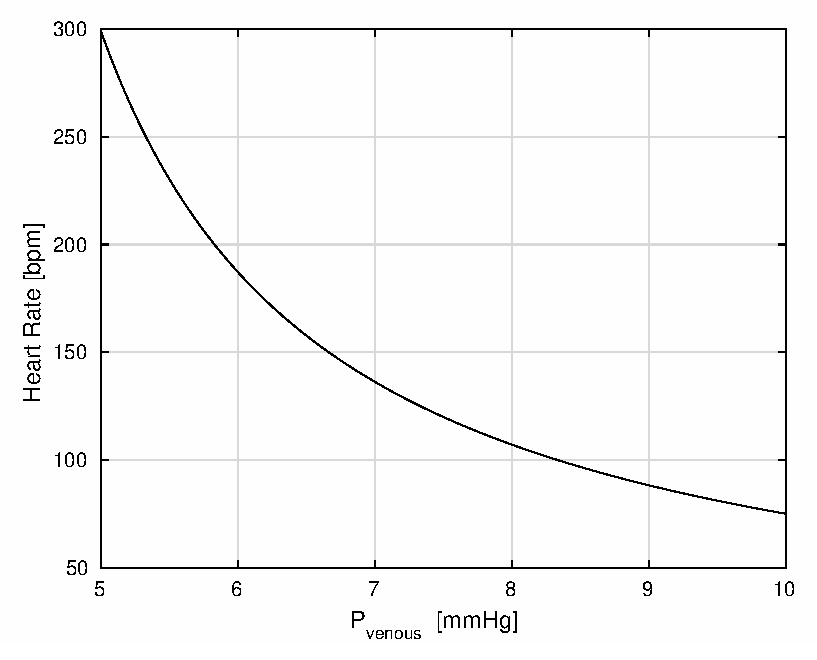
\includegraphics [width=4in]{Q2_01.eps}


\vspace{30pt}

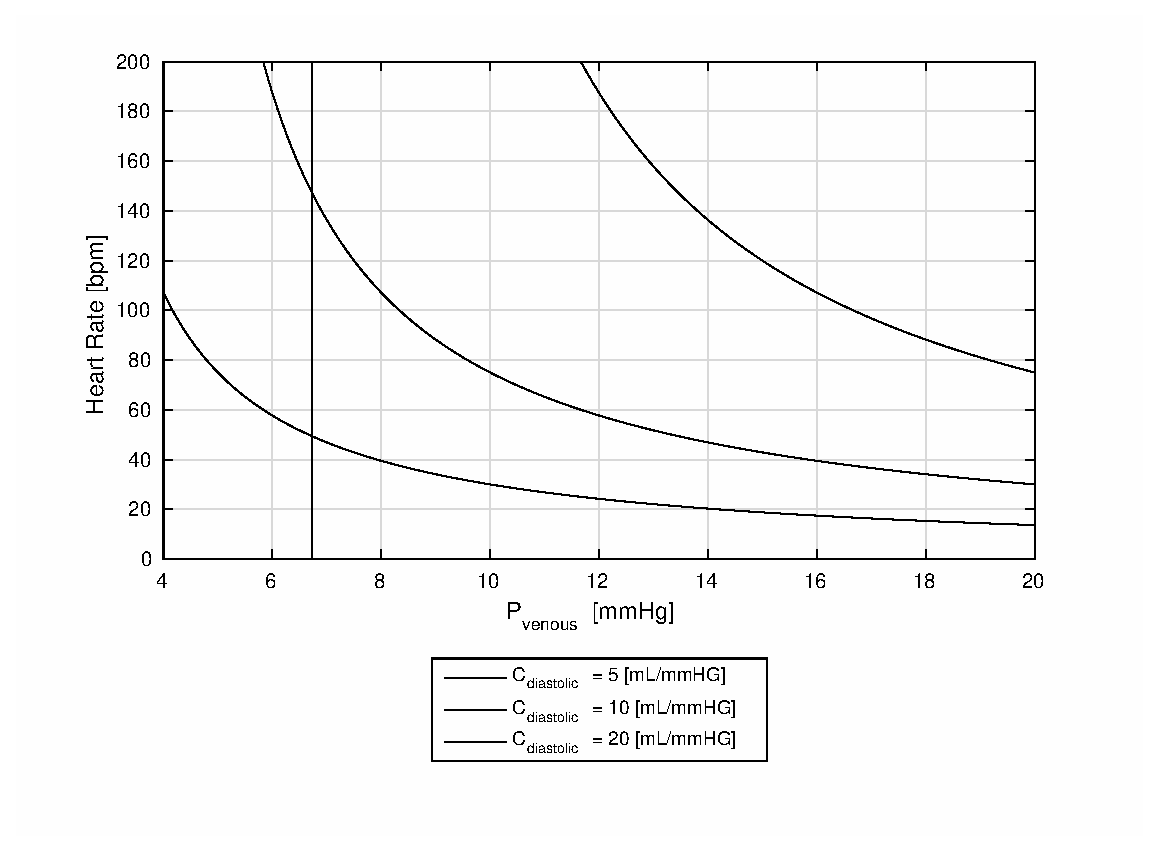
\includegraphics [width=4in]{Q2_02.eps}



\end{document}
    
